\documentclass[compress,xcolor=dvipsnames,10pt]{beamer}
\useoutertheme{smoothbars}
%\useoutertheme{miniframes}
\setbeamercovered{transparent}
\useoutertheme{infolines}
\useinnertheme[shadow=true]{rounded}
%%\usecolortheme{orchid}
%\usecolortheme{whale}

\usetheme{CambridgeUS}
\usecolortheme{beaver}
\setcounter{tocdepth}{2} % depth of the table of contents

\usepackage{moreverb}
\usepackage{verbatim}
%\usepackage{tikz}
%\usetikzlibrary{trees}
\usepackage{multirow}
\usepackage{xspace}



%

\newcommand{\ed}[2]{#1 \rightarrow #2}
\newcommand{\rr}[1]{\textcolor{red}{#1}}

\usepackage{color}
\usepackage{amsmath}
\usepackage{amssymb}
\usepackage{fancybox} % for shadow box and others type of boxes
\usepackage{graphicx} % for includegraphics
\usepackage{graphicx,color} % color
\usepackage{moreverb}
\usepackage{epsfig} % for include epsfig
\usepackage{subfigure}
\setbeamercovered{transparent} 
\usepackage{multirow}
%\usepackage{bera}
%\usepackage{algpseudocode}
\usepackage{algorithm}



\definecolor{dkgreen}{rgb}{0,0.6,0}
\definecolor{gray}{rgb}{0.5,0.5,0.5}
\definecolor{gray97}{gray}{.97}
\definecolor{gray45}{gray}{.45}
\definecolor{gray75}{gray}{.75}
\definecolor{mauve}{rgb}{0.58,0,0.82}
\definecolor{blueb}{rgb}{0,0,1}
\definecolor{redb}{rgb}{0.5,0,0}
\definecolor{darkblue}{rgb}{0.0,0.0,0.6}
\definecolor{cyan}{rgb}{0.0,0.6,0.6}

\usepackage{listings}


%Style Console
\lstdefinestyle{console}
{basicstyle=\scriptsize\bf\ttfamily
}

\lstdefinestyle{Bash}
{language=bash,
keywordstyle=\color{blue},
basicstyle=\ttfamily\scriptsize,
morekeywords={gcc, g++, jaber@jaber,cat,mkdir, ln, ls, grep, wc,cd, killall, top, vi, vim, tail, sudo, apt-get,pstree,make},
morekeywords=[2]{jaber@jaber:},
mathescape=false,
keywordstyle=[2]{\color{red}},
literate={\$}{{\textcolor{red}{\$}}}1 
         {:}{{\textcolor{red}{:}}}1
         {~}{{\textcolor{red}{\textasciitilde}}}1,
}

\lstdefinestyle{customc}
{language=C,
keywordstyle=\color{blue},
basicstyle=\ttfamily\scriptsize,
morekeywords={then, endif, endwhile, begin, end},
morekeywords=[2]{jaber@jaber:},
mathescape=false,
keywordstyle=[2]{\color{red}}
}


\lstdefinestyle{customjava}
{language=java,
keywordstyle=\color{blue},
basicstyle=\ttfamily\scriptsize,
morekeywords={String},
mathescape=true,
escapeinside={/*@}{@*/},
commentstyle=\color{dkgreen},   % comment style
keywordstyle=[2]{\color{red}}
}


\lstset{ %
style=customc,                % choose the language of the code
basicstyle=\tiny,       % the size of the fonts that are used for the code
numberstyle=\tiny,      % the size of the fonts that are used for the line-numbers
frame=Ltb,
rulesep=.4pt,
mathescape, % Allows escaping to (La)TeX mode within $$,
stringstyle=\color{redb},
showstringspaces = false,
basicstyle=\scriptsize\ttfamily,
keywordstyle=\color{darkblue}\bf,
 commentstyle=\color{dkgreen},   % comment style
%
breaklines=true
}


\newenvironment{remark}{{\bf\textcolor{Gray}{Remark
%\arabic{def}
    \,}}}
{\textcolor{Gray}{{\ \hfill $\Box$\\ 
%\stepcounter{def}
}}}

\newcommand{\blue}[1]{\textcolor{blue}{#1}}
\newcommand{\red}[1]{\textcolor{red}{#1}}
\newcommand{\green}[1]{\textcolor{green}{#1}}
\newcommand{\true}{\texttt{true}}
\newcommand{\false}{\texttt{false}}

\newcommand{\imp}{\Rightarrow}
\newcommand{\ev}{\equiv}
\newcommand{\notincluded}{\textcolor{red}{NOT INCLUDED}}

\newlength{\tablesepp}
\setlength{\tablesepp}{0.05in}

\newcommand{\ind}{\hspace*{1.5em}}
\newcommand{\T}{\mbox{\rm T}}
\newcommand{\F}{\mbox{\rm F}}
\newcommand{\AND}{\textbf{and }}

%% LOGICAL QUANTIFIERS
\newcommand{\A}{\ensuremath{\mathbf{\forall}}}
\newcommand{\E}{\ensuremath{\exists}}
\newcommand{\LQ}{\mbox{${\bf LQ}$}\xspace}


%% ARITHMETIC QUANTIFIERS
\renewcommand{\S}{\ensuremath{\Sigma}}
\renewcommand{\P}{\ensuremath{\Pi}}
\newcommand{\N}{\mbox{${\bf N}$}\xspace}
\newcommand{\AQ}{\mbox{${\bf AQ}$}\xspace}
\newcommand{\MAX}{\mbox{${\bf MAX}$}\xspace}
\newcommand{\MIN}{\mbox{${\bf MIN}$}\xspace}

%% QUANTIFIERS
\newcommand{\Q}{\mbox{${\bf Q}$}\xspace}
\newcommand{\q}{\mbox{${\bf q}$}\xspace}

%% MISC MATH SYMBOLS

\renewcommand{\l}{\ell}
\newcommand{\un}{\cup}
\newcommand{\union}{\bigcup}
\newcommand{\htp}[3]{\{#1\}\,#2\,\{#3\}}
\newcommand{\htptc}[3]{\langle#1\rangle\,#2\,\langle#3\rangle}
\newcommand{\la}{\langle}
\newcommand{\ra}{\rangle}
\newcommand{\var}{\mbox{$\varphi$}\xspace}
\newcommand{\cat}{\bullet}

 

\newcommand \orange[1]{{\color{orange}{#1}}}

\newcommand\demo[1]{
  \begin{flushright}
\orange{    \framebox{\textsc{demo: }#1}}
  \end{flushright}
}

\hypersetup{colorlinks=true,urlcolor=blue}

\AtBeginSection[]{
  \frame<handout:0>{
    \tableofcontents[current,currentsection]
  }
}

\color{darkblue}\bf

%% PROGRAMMING LANGUAGE SYNTAX
\newcommand{\IF}{{\color{darkblue}\bf if}\xspace}
\newcommand{\THEN}{{\color{darkblue}\bf then}\xspace}
\newcommand{\ELSE}{{\color{darkblue}\bf else}\xspace}
\newcommand{\ENDIF}{{\color{darkblue}\bf endif}\xspace}
\newcommand{\WHILE}{{\color{darkblue}\bf while}\xspace}
\newcommand{\DO}{{\color{darkblue}\bf do}\xspace}
\newcommand{\ENDWHILE}{{\color{darkblue}\bf endwhile}\xspace}
\newcommand{\BEGIN}{{\color{darkblue}\bf begin}\xspace}
\newcommand{\END}{{\color{darkblue}\bf end}\xspace}
\newcommand{\PROC}{{\color{darkblue}\bf procedure}\xspace}
\newcommand{\CALL}{{\color{darkblue}\bf call}\xspace}
\newcommand{\VAL}{{\color{darkblue}\bf value}\xspace}
\newcommand{\VALRES}{{\color{darkblue}\bf value-result}\xspace}
\newcommand{\RES}{{\color{darkblue}\bf result}\xspace}


%%%% General %%%%
\renewcommand{\ss}{\smallskip}
\newcommand{\Eg}{E.g.,\xspace}
\newcommand{\eg}{e.g.,\xspace}
\newcommand{\ie}{i.e.,\xspace}


\newcommand{\codetext}[1]{\texttt{#1}\xspace}
\newcommand{\optext}[1]{\texttt{#1}}


%%% DATA SETS
\newcommand{\Cl}{\codetext{Class}\xspace}
\newcommand{\Cn}{\codetext{CourseName}\xspace}
\newcommand{\Cr}{\codetext{Course}\xspace}
\newcommand{\En}{\codetext{Entries}\xspace}
\newcommand{\Gd}{\codetext{Grade}\xspace}
\newcommand{\Id}{\codetext{IdNum}\xspace}
\newcommand{\Mj}{\codetext{Major}\xspace}
\newcommand{\Nm}{\codetext{Name}\xspace}
\newcommand{\St}{\codetext{Student}\xspace}
\newcommand{\Sm}{\codetext{Semester}\xspace}
\newcommand{\Tn}{\codetext{Transcript}\xspace}


\newcommand{\actid}[1]{\ensuremath{\mathsf{#1}}\xspace}
\newcommand{\cd}[1]{\codetext{#1}}
\newcommand{\ct}[1]{\textsc{#1}}


\newcommand{\emp}[1]{\textbf{#1}}
\newcommand{\empp}[1]{\emph{#1}}
\newcommand{\empb}[1]{\textbf{#1}}
\newcommand{\empi}[1]{\textit{#1}}
\newcommand{\empbi}[1]{\textbf{\textit{#1}}}

\newcommand{\satt}{\equiv}
\newcommand{\sat}{\models}



%%%%%%%%%%%%%%%%%%%%%%%%%%%%%%%%%%%%%%%%%%%%%%%%%%%%%%%%%%%%%%%%%%%%%%
%%%%%%%%%%%%%%% Key Emphasized Terms ``Michael Jackson style''

\newcommand{\fundterm}[1]{\textsc{#1}\xspace}
\newcommand{\plural}[1]{{#1}\fundterm{s}}

\newcommand{\actions}{\fundterm{actions}}
\newcommand{\act}{\fundterm{action}}
\newcommand{\acts}{\fundterm{actions}}
\newcommand{\app}{\fundterm{application}}
\newcommand{\appdom}{\fundterm{application domain}}
\newcommand{\appsoft}{\fundterm{application software}}
\newcommand{\aut}{\fundterm{automaton}}
\newcommand{\auts}{\fundterm{automata}}
\newcommand{\Buchi}{\fundterm{Buchi automaton}}
\newcommand{\Buchis}{\fundterm{Buchi automata}}
\newcommand{\comp}{\fundterm{computation}}
\newcommand{\comps}{\plural{\comp}}
\newcommand{\checks}{\fundterm{checks}}
\newcommand{\checksclause}{\fundterm{checks clause}}
\newcommand{\datmod}{\fundterm{data model}}
\newcommand{\datmods}{\plural{\datmod}}
\newcommand{\decomposed}{\fundterm{decomposed}}
\newcommand{\defnn}{\fundterm{definition}}
\newcommand{\defnns}{\plural{\defnn}}
\newcommand{\desc}{\fundterm{description}}
\newcommand{\descs}{\fundterm{descriptions}}
\newcommand{\desig}{\fundterm{designation}}
\newcommand{\desigs}{\plural{\desig}}
\newcommand{\design}{\fundterm{design}}
\newcommand{\effects}{\fundterm{effects}}
\newcommand{\effectsclause}{\fundterm{effects clause}}
\newcommand{\event}{\fundterm{event}}
\newcommand{\events}{\fundterm{events}}
\newcommand{\globc}{\fundterm{global constraint}}
\newcommand{\globcs}{\fundterm{global constraints}}
\newcommand{\helps}{\fundterm{helps}}
\newcommand{\impl}{\fundterm{implementation sketch}}
\newcommand{\interface}{\fundterm{interface}}
\newcommand{\interfaces}{\fundterm{interfaces}}
\newcommand{\mach}{\fundterm{machine}}
\newcommand{\machine}{\fundterm{machine}}
\newcommand{\model}{\fundterm{model}}
\newcommand{\module}{\fundterm{module}}
\newcommand{\modules}{\fundterm{modules}}
\newcommand{\modint}{\fundterm{module interface}}
\newcommand{\modints}{\fundterm{module interfaces}}
\newcommand{\modifies}{\fundterm{modifies}}
\newcommand{\modspec}{\fundterm{module specification}}
\newcommand{\modspecs}{\fundterm{module specifications}}
\newcommand{\overview}{\fundterm{overview}}
\newcommand{\precond}{\fundterm{precondition}}
\newcommand{\postcond}{\fundterm{postcondition}}
\newcommand{\probcntxt}{\fundterm{problem context}}
\newcommand{\program}{\fundterm{program}}
\newcommand{\programs}{\fundterm{programs}}
\newcommand{\reqs}{\fundterm{requirements}}
\newcommand{\requires}{\fundterm{requires}}
\newcommand{\requiresclause}{\fundterm{requires clause}}
\newcommand{\requirements}{\fundterm{requirements}}
\newcommand{\spec}{\fundterm{specification}}
\newcommand{\scopes}{\fundterm{scopes}}
\newcommand{\state}{\fundterm{state}}
\newcommand{\states}{\plural{\state}}
\newcommand{\stspc}{\fundterm{state space}}

%%%%%%%%%%%%%%%%%%%%%%% GENERAL MATH SYMBOLS %%%%%%%%%%%%%%%%%%%%%%%%%%%%%%

\newcommand{\Adj}{\mathop{\rm Adj}\nolimits}
\newcommand{\abs}[1]{\left| #1\right|}
\newcommand{\card}[1]{\left| #1\right|}
\newcommand{\ar}{\rightarrow}  
%\newcommand{\ar}{\longrightarrow}
\newcommand{\al}{\alpha}
\renewcommand{\b}[1]{\overline{#1}}
\newcommand{\choice}{\mbox{$[\hspace*{-1.0pt}]$}}
\newcommand{\ceil}[1]{\left\lceil #1 \right\rceil}
\renewcommand{\d}{\, . \,}      % separator in quantified formulae
\newcommand{\df}{\triangleq}
%\newcommand{\df}{\mbox{$\:\stackrel{\rm df}{=\!\!=}\:$}}
\newcommand{\dn}{\mbox{$\hspace{-0.1em}\downarrow\hspace{-0.1em}$}}
\newcommand{\Ex}{\mathop{\rm Ex}}
\newcommand{\es}{``"}   %empty string
\newcommand{\expect}[1]{{\rm E}\left[ #1 \right]}
\newcommand{\expectsq}[1]{{\rm E}^2\left[ #1 \right]}
\newcommand{\floor}[1]{\left\lfloor #1 \right\rfloor}
\renewcommand{\ge}{\geqslant}
\newcommand{\given}{\mid}
\newcommand{\halfind}{\hspace*{1.5em}}
\newcommand{\ifof}{\Longleftrightarrow} % logical equivalence
\newcommand{\img}{\mathrm{Image}}
\newcommand{\ints}{\cap}
\renewcommand{\l}{\ell}
\renewcommand{\le}{\leqslant}
\newcommand{\lra}{\mbox{$\longrightarrow$}}
%\newcommand{\mod}{\ \mathrm{mod}\ }
\newcommand{\oneton}{\{1,\,\ldots, n\}}
\newcommand{\paren}[1]{\left( #1 \right)}
\newcommand{\prob}[1]{\Pr\left\{ #1 \right\}}
\newcommand{\pind}{\hspace*{3.0em}}
\newcommand{\pj}{\!\upharpoonright\!}
\newcommand{\proj}{\pj}
\newcommand{\preimg}{\mathrm{PreImage}}
\newcommand{\pl}{\!\parallel\!}
\newcommand{\s}{\mbox{$\hspace{-1pt}-\hspace{-2pt}$}}
\newcommand{\set}[1]{\left\{ #1 \right\}}
%\newcommand{\set}[1]{\{#1\}}
\newcommand{\seq}{\approx}
\newcommand{\spc}{\mbox{\vspace{-0.25in}}}
\newcommand{\sct}{\ensuremath{\ |\ }}
\newcommand{\st}[2]{\mbox{$\stackrel{#1}{#2}$}} % abbreviated stackrel}
%\newcommand{\st}{\ | \ }
\newcommand{\sub}{\subseteq}
\newcommand{\twodots}{\mathinner{\ldotp\ldotp}}
\newcommand{\tiff}{\textup{\ iff\ }}
\newcommand{\tl}[1]{\mbox{$\tilde{#1}$}}% abbreviated tilde
\newcommand{\tpl}[1]{\ensuremath{\langle #1 \rangle}}
\newcommand{\up}{\mbox{$\hspace{-0.1em}\uparrow\hspace{-0.1em}$}}
\newcommand{\Var}{\mathop{\rm Var}\nolimits}
\newcommand{\variance}[1]{{\rm Var}\left[ #1 \right]}
\newcommand{\w}{\omega}                


%%%%%%%%%%%%%%%%%%% Ints, Reals, etc %%%%%%%%%%%%%%%%%%%%%%%%%%%%%

\newcommand{\reals}{{\mathbb R}}
\newcommand{\integers}{{\mathbb Z}}
\newcommand{\naturals}{{\mathbb N}}
\newcommand{\nat}{\naturals}
\newcommand{\nats}{\naturals}
\newcommand{\rationals}{{\mathbb Q}}
\newcommand{\complex}{{\mathbb C}}
\newcommand{\complexes}{{\mathbb C}}



%%%%%%%%%%%%%%%%%%%%%%%%% MATH MACROS AND ENVIRONMENTS %%%%%%%%%%%%%%%%%%%%%%%%%%

%\newcommand{\se}[3]{\ensuremath{#1[#2 .. #3]}}
\newcommand{\se}[3]{\ensuremath{#1[#2 \! : \! #3]}}
%\newcommand{\se}[3]{\ensuremath{#1[#2,\ldots,#3]}}



%%%%%%%%%%%%%%%%%%%%%%%%%%%%%%%%%%%%%%%%%%%%%%%%%%%%%%%%%%%%%%
%%%%%%%%%%%%%%%%% START IntSet EXAMPLE %%%%%%%%%%%%%%%%%%%%%%%

\newcommand{\els}{\ensuremath{els}\xspace}
\newcommand{\elsa}{\ensuremath{els}}
\newcommand{\gI}{\codetext{getIndex}\xspace}
\newcommand{\insrt}{\codetext{insert}}
\newcommand{\isIn}{\codetext{isIn}}
\newcommand{\IntSet}{\codetext{IntSet}}
\newcommand{\IntSetNoDup}{\codetext{IntSetNoDup}\xspace}
\newcommand{\IntSetNoDupSort}{\codetext{IntSetNoDupSort}\xspace}
\newcommand{\IntSetSort}{\codetext{IntSetSort}\xspace}
\newcommand{\remov}{\codetext{remove}}
\newcommand{\ISunion}{\codetext{union}} %% union --> ISunion
\newcommand{\sze}{\codetext{size}\xspace}
\renewcommand{\top}{\ensuremath{top}\xspace}

%%%%%%%%%%%%%%%%% IntSet iterator
\newcommand{\elements}{\codetext{elements}\xspace}
\newcommand{\IntGenerator}{\codetext{IntGenerator}}

%%%%%%%%%%%%%%%%% END IntSet EXAMPLE %%%%%%%%%%%%%%%%%%%%%%%
%%%%%%%%%%%%%%%%%%%%%%%%%%%%%%%%%%%%%%%%%%%%%%%%%%%%%%%%%%%%%%



%%%%%%%%%%%%%%%%%%%%%%%%%%%%%% Misc Abbrevs %%%%%%%%%%%%%%%%%%%%%%%%%%%%%%%%%%%

%\newcommand{\spec}{\textsf}     % use for problem specification

\newcommand{\AF}{\mathrm{AF}}
\newcommand{\repok}{\texttt{repOk}\xspace}
\newcommand{\intset}{\mathrm{set}}
\newcommand{\aop}{\mathtt{abstract\!-\!op}}
\newcommand{\cop}{\mathtt{concrete\!-\!op}}

\newcommand{\inv}{\ensuremath{\!\sim\!}}


%%%%%%%%%%%%%%%%%% JAVA keywords in teletype code style
\newcommand{\Iterator}{\codetext{Iterator}}
\newcommand{\generator}{\codetext{generator}\xspace}
\newcommand{\hasNext}{\codetext{hasNext}\xspace}
\newcommand{\java}{\codetext{java}}
\newcommand{\util}{\codetext{util}}
\newcommand{\Object}{\codetext{Object}\xspace}
\newcommand{\Integer}{\codetext{Integer}\xspace}
\newcommand{\intValue}{\codetext{intValue}\xspace}















\begin{document}
%%%%%%%%%%%%%%
\graphicspath{{figs/}}
\subtitle{Behaviors and Conversations}
\title[Java-Based BIP]{Java-Based BIP}
\author[]{}
 \institute[]{}
\date[]{}


\begin{frame}
 \maketitle
\end{frame}
%%%%%%%%%%%%%%


\begin{frame}[fragile]
\frametitle{Base Components (Behaviors)}
\begin{columns}
 \begin{column}{0.4\linewidth}
 \begin{center}
 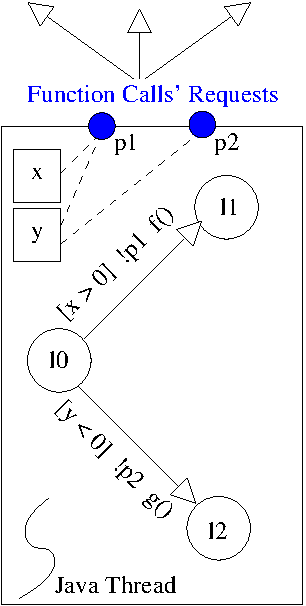
\includegraphics[scale=0.5]{figs/basecomponent.pdf}
\end{center}
  \end{column}
   \begin{column}{0.55\linewidth}
   \begin{lstlisting}[style=customjava, basicstyle=\ttfamily\tiny]
public class ExampleComp extends BaseComponent {
  private WrapInt x = new WrapInt();
  private WrapInt y = new WrapInt();
  
  // Locations
  private Location l0 = new Location();
  private Location l1 = new Location();
  private Location l2 = new Location();
   
  // Ports
  public SendPort p1 = new SendPort(x, y);
  public SendPort p2 = new SendPort(y);
  public ExampleComp(Compound compound) {
    super(compound);
    setInitial(l0);
    
    addTransition( new Transition(l0, l1, p1) {
      public boolean guard()  { return x.value > 0; }
      public void action()    { x.value++; }
    });
     
    addTransition( new Transition(l0, l2, p2) {
      public boolean guard()  { return y.value < 0; }
      public void action()    { y.value += x.value; }
    });
  }
}
\end{lstlisting}
  \end{column}
 \end{columns}
\end{frame}

\begin{frame}[fragile]
\frametitle{Synchronization Components (Conversations)}
\begin{columns}
 \begin{column}{0.45\linewidth}
  \begin{center}
 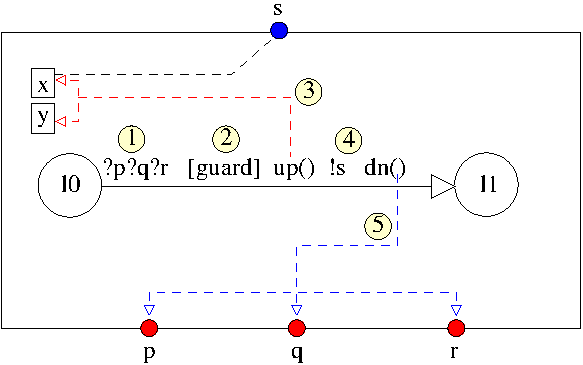
\includegraphics[scale=0.5]{figs/synccomponent.pdf}
\end{center}
  \end{column}
   \begin{column}{0.55\linewidth}
   \begin{lstlisting}[style=customjava, basicstyle=\ttfamily\tiny]
public class ExampleSync extends SyncComponent {
  private WrapInt x = new WrapInt();
  private WrapInt y = new WrapInt();
  
  // Locations
  private Location l0 = new Location();
  private Location l1 = new Location();
   
  // Ports
  public SendPort s = new SendPort(x);
  
  public ReceivePort p = new ReceivePort();
  public ReceivePort q = new ReceivePort();
  public ReceivePort r = new ReceivePort();

  public ExampleSync(Compound compound) {
    super(compound);
    setInitial(l0);
    
    addTransition( new Transition(l0, l1, s, p, q, r) {
      public boolean guard()  { 
        return ((WrapInt)p.getVariable(0)).value 
            <= ((WrapInt) q.getVariable(0)).value;
      }
      public void up() { 
        x.value = ((WrapInt) p.getVariable(0)).value; 
      }
      public void dn() { 
        ((WrapInt) q.getVariable(1)).value = x + y; 
      }
    });
  }
}
\end{lstlisting}
  \end{column}
 \end{columns}
\end{frame}

\begin{frame}
 \frametitle{Behaviors and Conversations}
 \begin{center}
  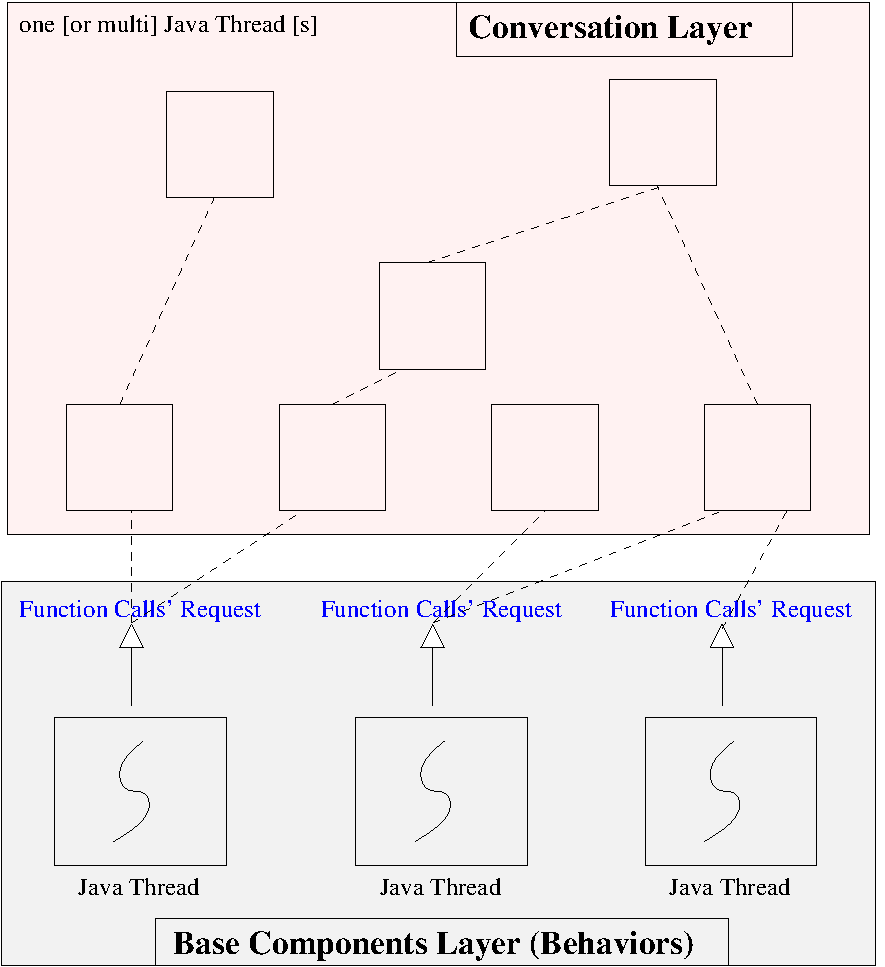
\includegraphics[scale=0.45]{figs/javabip.pdf}
 \end{center}

\end{frame}



\begin{frame}[fragile]
 \frametitle{Implementation}
 \begin{itemize}
  \item Thread per base component.
  \item Thread for the conversation layer.
 \end{itemize}

\end{frame}


\begin{frame}[fragile]
 \frametitle{Implementation - Base Component}

       \begin{lstlisting}[style=customjava, basicstyle=\ttfamily\tiny]
public void run() {
  while(true) {
    try {
      notifyConversationLayer();
      semaphore.acquire();
    }
    catch (InterruptedException e) {
       return; // An interrupt has been sent from the conversation, in case of global deadlock. 
    }
    performTransition();
  }
}
\end{lstlisting}
\begin{enumerate}
\item Notify the conversation layer, that is:
\begin{enumerate}
\item Check the guard of the outgoing transitions 
\item Notify the corresponding receive ports accordingly
\begin{enumerate}
 \item Mark each receive port (of a specific sync component) as been notified
 \item Check if there exist a transition where all its receive ports have been notified and its guard is \texttt{true}
 \item Execute the \texttt{up()} method and keep track of the selected transition
 \item If that transition has a send port, then notify the corresponding receive ports, and so on
\end{enumerate}
\item Increment the value of the conversation layer semaphore
\end{enumerate}
\item Wait for the conversation layer (if an interrupt has been received return) 
\item On resume, execute the corresponding action of the transition and move to the next location
\end{enumerate}

\end{frame}



\begin{frame}[fragile]
 \frametitle{Implementation - Conversation Layer}

       \begin{lstlisting}[style=customjava, basicstyle=\ttfamily\tiny]
public void run() {
  while(true) {
    waitComponents();
    compute();
    if(!thread.isInterrupted())
      notifyComponents();
    else {
      System.out.println("***** deadlock ******");
      return;
    }
  }
}
\end{lstlisting}
\begin{enumerate}
\item Wait for all the base components
\item Compute, that is
\begin{enumerate}
\item Select a radom sync component which is ready and in the top (i.e., the selected transition has no send port)
\item If such component does exist:
\begin{enumerate}
 \item Execute the down action of the selected sync component and change its location
\item Recursively execute the down action of the bottom sync components and move the locations accordingly. 
\item If the bottom component is a base component store its corresponding send port   
\end{enumerate}
\item otherwise, global deadlock detection, send an interrupt to the base components and myself 
\end{enumerate}
\item If not interrupted, notify the base components (i.e., release their semaphores set their port to be executed), otherwise return 
\end{enumerate}

\end{frame}


\begin{frame}
 \frametitle{Example: Network Sorting Algorithm (version 1)}
 \begin{center}
  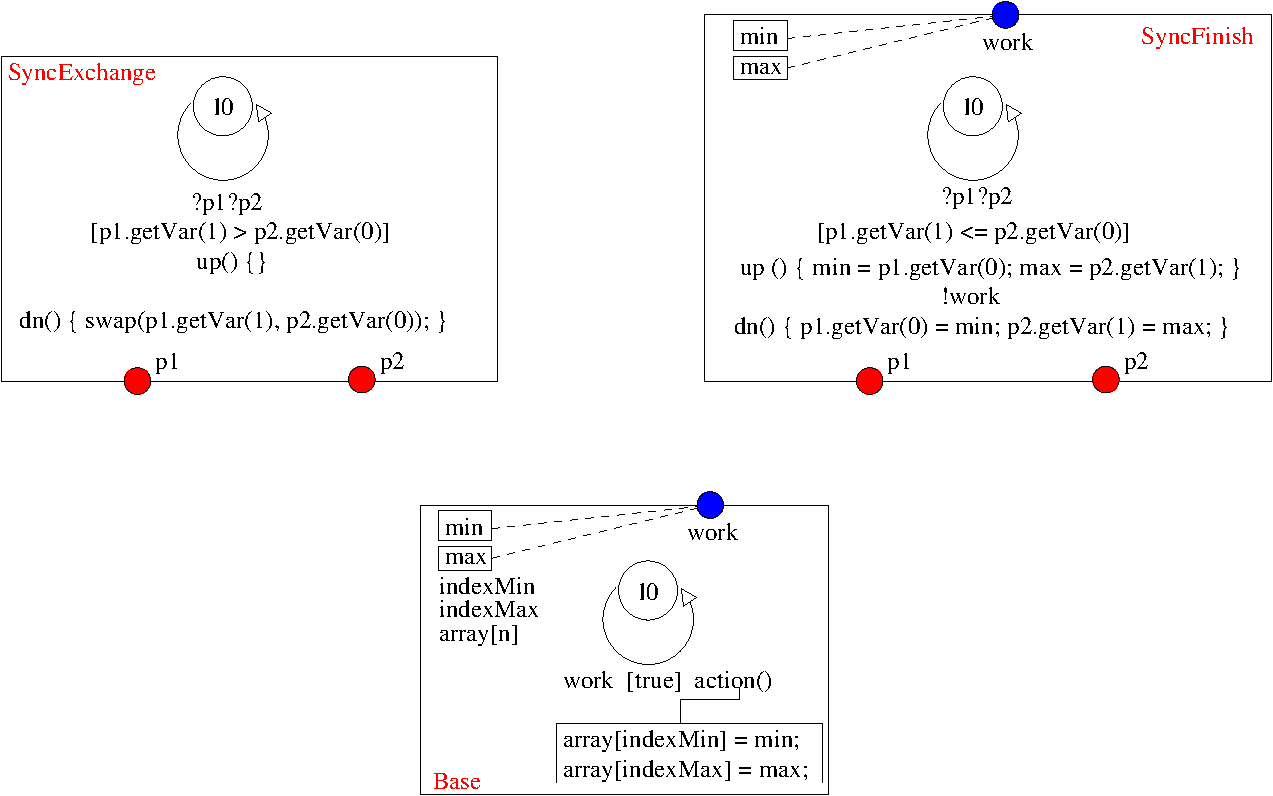
\includegraphics[scale=0.45]{figs/nsa1v1.pdf}
 \end{center}

\end{frame}


\begin{frame}
 \frametitle{Example: Network Sorting Algorithm (version 1)}
 \begin{center}
  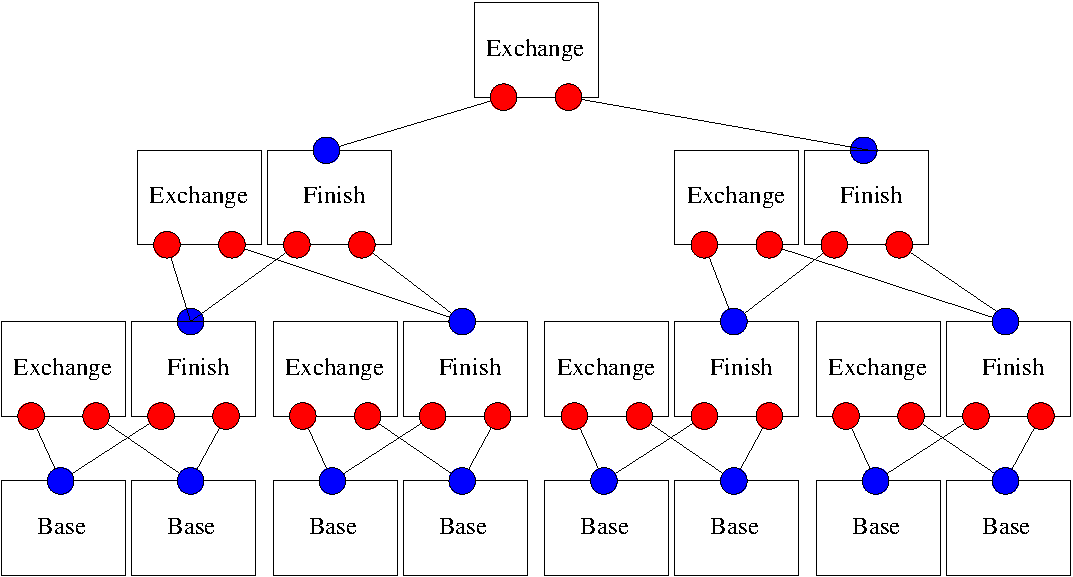
\includegraphics[scale=0.45]{figs/nsa2v1.pdf}
 \end{center}
 \end{frame}
 
 \begin{frame}
 \frametitle{Example: Network Sorting Algorithm (version 2)}
 \begin{center}
  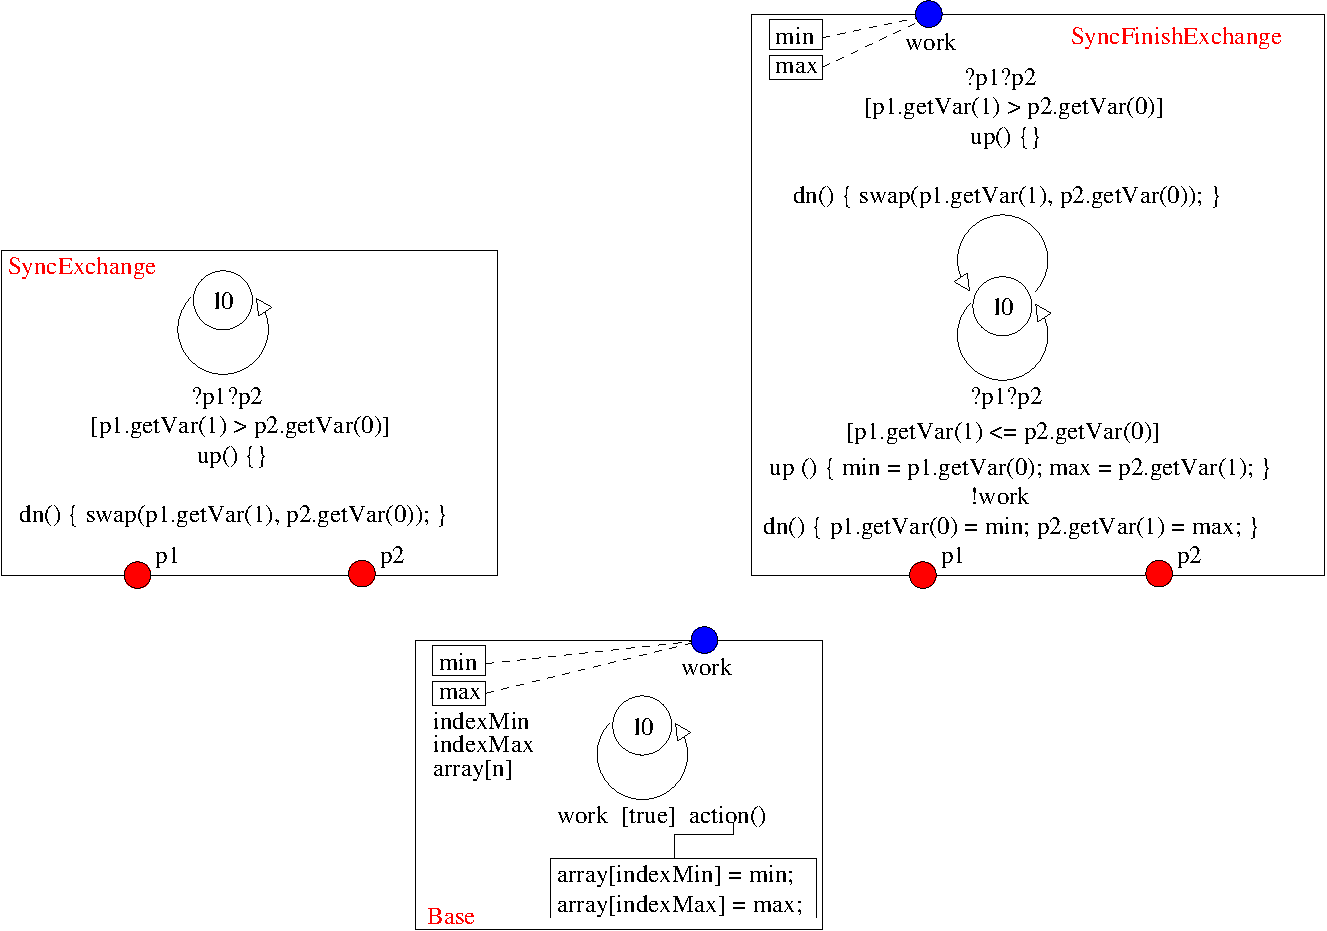
\includegraphics[scale=0.45]{figs/nsa1v2.pdf}
 \end{center}
\end{frame}


\begin{frame}
 \frametitle{Example: Network Sorting Algorithm (version 2)}
 \begin{center}
  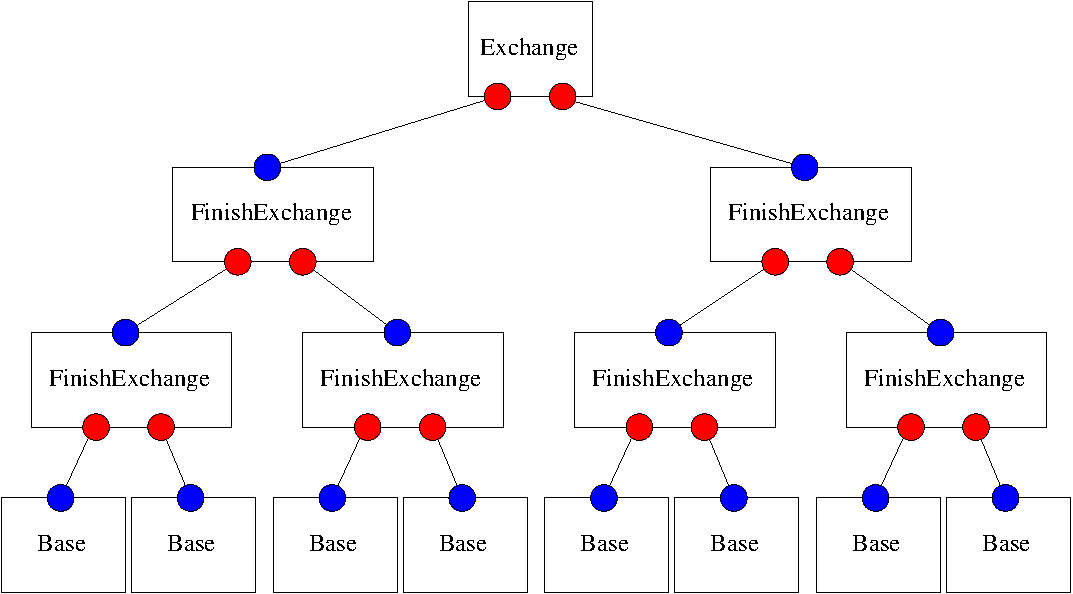
\includegraphics[scale=0.45]{figs/nsa2v2.pdf}
 \end{center}
\end{frame}

\begin{frame}[fragile]
 \frametitle{Example: Network Sorting Algorithm (version 2)}
        \begin{lstlisting}[style=customjava, basicstyle=\ttfamily\tiny]
// Base Components
ArrayAtom comp1 = new ArrayAtom(this, 10);
ArrayAtom comp2 = new ArrayAtom(this, 10);
ArrayAtom comp3 = new ArrayAtom(this, 10);
ArrayAtom comp4 = new ArrayAtom(this, 10);
ArrayAtom comp5 = new ArrayAtom(this, 10);
ArrayAtom comp6 = new ArrayAtom(this, 10);
ArrayAtom comp7 = new ArrayAtom(this, 10);
ArrayAtom comp8 = new ArrayAtom(this, 10);

// Sync Components
ExchangeFinish sync1 = new ExchangeFinish(this);
ExchangeFinish sync2 = new ExchangeFinish(this);
ExchangeFinish sync3 = new ExchangeFinish(this);
ExchangeFinish sync4 = new ExchangeFinish(this);
ExchangeFinish sync5 = new ExchangeFinish(this);
ExchangeFinish sync6 = new ExchangeFinish(this);

Exchange top = new Exchange(this);

// Connections
sync1.p1.connect(comp1.work);
sync1.p2.connect(comp2.work);
sync2.p1.connect(comp3.work);
sync2.p2.connect(comp4.work);
sync3.p1.connect(comp5.work);
sync3.p2.connect(comp6.work);
sync4.p1.connect(comp7.work);
sync4.p2.connect(comp8.work);

sync5.p1.connect(sync1.work);
sync5.p2.connect(sync2.work);
sync6.p1.connect(sync3.work);
sync6.p2.connect(sync4.work);

top.p1.connect(sync5.work);
top.p2.connect(sync6.work);
\end{lstlisting}
\end{frame}


\begin{frame}
\frametitle{Restrictions - No Cycle}
\begin{columns}
\begin{column}{0.4\textwidth}
\begin{center}
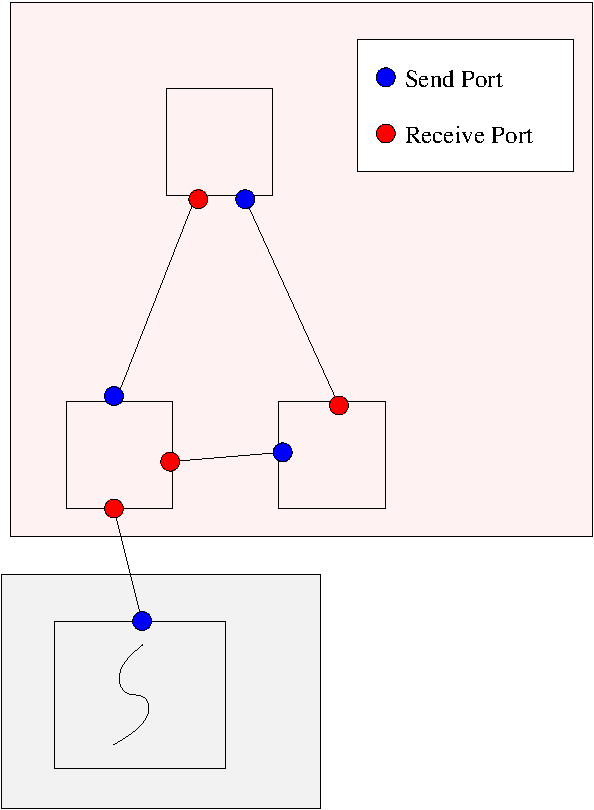
\includegraphics[scale=0.35]{restrictionNoCycle.pdf}
\end{center}
\end{column}
\begin{column}{0.6\textwidth}
Note that, the static connections may contain a cycle but at runtime this cycle is not reachable. 
\begin{block}{TODO}
For safety, avoid connections that may lead to a cycle. That is, check if the static connections contain a deadlock, if so, throw an exception.  
\end{block}
\end{column}
\end{columns}

\end{frame}



\begin{frame}
\frametitle{Restrictions - Deterministic Sync Components}

\begin{center}
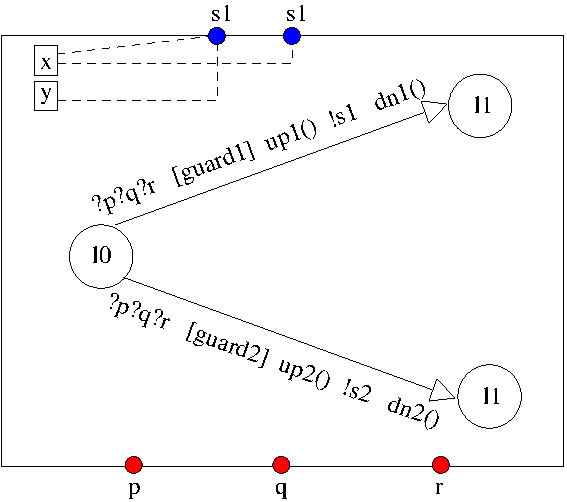
\includegraphics[scale=0.35]{deterministicSync.pdf}
\end{center}

\begin{itemize}
\item We assume that sync component are deterministic. That is, from the current location, at maximum one of the outgoing transition could be ready.
\item If not, we need to propagate up different value for each variable which is not to obvious. 
\item Under this assumption, upon find a ready transition (all ports received, it guard is true), we can directly notify the corresponding receive ports. 
\item If the propagation will not lead to an enable top sync component, it will not be a problem because of the assumption we have. 
\item In the worst case, we can assume that the behavior of the sync component with no choice, or with choice but with mutually exclusive guards.  
\end{itemize}
 
\end{frame}


\begin{frame}
\frametitle{Restrictions - Conflict Intersection}
\begin{columns}
\begin{column}{0.4\textwidth}
\begin{center}
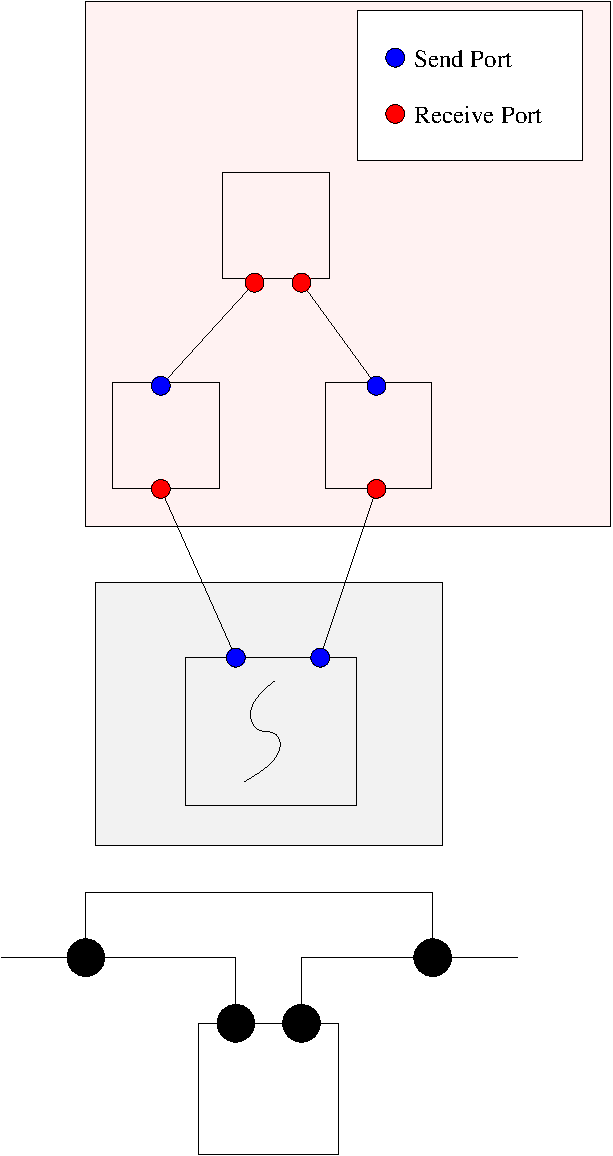
\includegraphics[scale=0.35]{restrictionIntersection.pdf}
\end{center}
\end{column}
\begin{column}{0.6\textwidth}
\begin{itemize}
\item The figures on the left may lead to a semantic violation. We can avoid such situation statically, as for the cycles. It will be too restrictive, because if the sync component on the top notifies only of is receive ports, in this case, it should be OK. 
\item Note that, sync components do not suffer from this problem, this is because we assume that are deterministic (see restriction above). 
\end{itemize}

\begin{block}{TODO}
However, at runtime, we should check if a component receives two different notifications within an execution cycle [\textcolor{green}{DONE}]. 
\end{block}
\end{column}
\end{columns}
\end{frame}


\begin{frame}
\frametitle{Conversation Layer - Possible Improvements}
Currently we are selecting one top component and the we notify the corresponding base components. 
\begin{block}{Choice 1}
\begin{enumerate}
\item Select a top sync component.
\item Down propagation to compute the corresponding send ports of base components.
\item For each base component that contains a selected send port, reset the other send ports for other outgoing transition from the current location.
\item Recheck if there are others top sync components. If so go to 1, otherwise notify all the send ports of the base components.  
\end{enumerate}
\end{block}

Following this scenario may improve the performance drastically [\textcolor{green}{DONE}]. 
\end{frame}

\begin{frame}
\frametitle{Conversation Layer - Possible Improvements}
\begin{block}{Choice 2}
\begin{itemize}
\item Conversation layer do not need to wait all the base components. 
\item After a base component does the up notifications, it checks if it it reaches a top sync component and ready. 
\item In that case, it can notify the conversation layer. 
\item While the conversation layer is propagating down, it disables all the corresponding sync components that are connected to those selected. 
\item That is, we do not need to notify all the base components as in the current implementation. 
\begin{itemize}
\item Some of the base components will be notified to execute some port
\item others will be notified by null in order to reset. This is because while propagating down we have disabled some of the sync components. 
\item The rest will still be waiting.  
\end{itemize}
\item Following this scenario may improve the performance drastically. ``This may contradict with the semantic proposed by Simon'' as it allows conflict on the same port.
\end{itemize}
\end{block}
\end{frame}

\begin{frame}
\frametitle{Conversation Layer - Possible Improvements}
\begin{block}{Choice 2}
\begin{itemize}
\item Partition sync component into groups. 
\item Create one thread per group. 
\item This may lead to some conflicts. 
\end{itemize}
\end{block}
\end{frame}

\newcommand{\goesto}[1][]{\stackrel{#1}{\longrightarrow}} % -->
\newcommand{\ngoesto}[1][]{\stackrel{#1}{\not\longrightarrow}} % -->
\newcommand{\arrow}[2]  {\xrightarrow[{\scriptsize #2}]{{\scriptsize #1}}}

\begin{comment}
\begin{frame}
\frametitle{Semantic Trash}
$$
\frac
{l \arrow{a/S}{} l' \quad q_1 \arrow{p_1}{X_1} a'_1 \quad q_2 \arrow{p_2}{X_2} a'_2 \quad a = p_1 p_2
}
{(l,q_1,q_2) \arrow{a/S}{X_1 \cup X_2 \cup S} (l', q'_1, q'_2)}
$$
$$
\cup_S \arrow{a}{}_S
$$
$$ Top
\frac
{\arrow{a/-}{}}
{(l,q_1,q_2) \arrow{a}{}_S (l', q'_1, q'_2)}
$$

$X$ set of components

$S$ a sync component

$$
(q_{\bar{X}}, q_X) \arrow{a}{}(q_{\bar{X}}, q'_X)
$$

$$
 q_X \arrow{a/-}{X} q'_X
$$
\end{frame}
\end{comment}

\begin{frame}
 \frametitle{Non-Deterministic Sync Components}
 \begin{itemize}
  \item Lower component: update function

\begin{itemize}
 \item Replace \texttt{value} of the wrappers by \texttt{value()} with a \texttt{private int index}
\item For each outgoing transition we assign an index
\item \texttt{value} will create a copy of the variable if it is not already create for the given index. 
\item The wrapper will eventually contains different copies of it. 
\item We set the \texttt{index}, then we call the update function. 
\item The \texttt{value()} method returns the value of the copy at the \texttt{index}
\end{itemize}
\end{itemize}

\end{frame}
\begin{frame}
 \frametitle{Non-Deterministic Sync Components}
 \begin{itemize}
  \item Upper component: guard
\begin{itemize}
 \item When receiving a notification that a port is ready on a specific transition. In practice we are receiving this port with some values.
 \item It is possible that, because of non-deterministic of the lower layer, we will receive a notification from the same port but with different values. 
 \item When all the received ports are notified of a transition, for all possible combinations (indices) of the available values, we evaluate the guard.
 \item If two variables belongs to the same component they should be assigned to the same index. 
 \item Upon receiving another notification (new values), we evaluate the received values with the existing ones. 
 \item For each variable copy we have the index of the transition and an index of the lower layer. Different solutions: 
 \begin{enumerate}
  \item N transitions $\implies$ N copies per variable. Upper M transitions $\implies$ N $\times$ M copies per variable [bad solution, too many variables], but we need to send only one index. 
  \item Create a copy only if necessary. Here two options exist (1) send an index per variable copy (2) when create a variable, fill in the other non created variables with their default values (then we can send only one index per send).  
 \end{enumerate}

\end{itemize}
 \end{itemize}
\end{frame}
\begin{frame}
 \frametitle{Non-Deterministic Sync Components}
 {\scriptsize
 Remark: If the lower component contains two outgoing transitions where both are labeled with send port $p_1$, and the upper component contains also two outgoing transitions both labeled with receive port $p_1$.
 So, in the worst case, we have to create four copies of the corresponding variables of the upper component (e.g., first upper transition receives $p_1$ of the first lower transition, first upper transition receives $p_1$ of the second lower transition, 
 Second upper transition receives $p_1$ of the first lower transition, and finally second upper transition receives $p_1$ of the second lower transition). We have to keep track of the selected transition at each layer. 
 Example:
 \scriptsize ?p1?p2?p3   !s1: p1 corresponds to a transition in the lower executed with some values (lower of the lower).
 }
\end{frame}

\begin{frame}
 \frametitle{Non-Deterministic Sync Components}
 \begin{enumerate}
 \item A transition is assigned to receive ports (e.g. $?p_1 \, ?p_2 \, ?p_3$).
  \item Each receive port is assigned to variables, where each variable has N copies. 
  \item When receiving all the receive ports of a given transition $t_i$, we execute its up action. 
  \item All the modifications of the variables should be done through the call of \texttt{value} method. 
  \item Calling \texttt{x.value()} method creates a copy the variable \texttt{x} at the current index. 
  \item The current index depends on the current transition and an index from the lower layer (an index from lower layers mimics the corresponding values of its variables). 
  \item If for a given current index we call \texttt{y.value()} such that for previouses current indices we do not create a copy of that variable, then we should fill them with the value of its original variable. 
 \item So that when a transition is enabled we notify the corresponding send port with a given index. 
 \end{enumerate}

\end{frame}


\end{document}
